\documentclass{article}
\usepackage{booktabs}
\usepackage{amsmath}
\usepackage[margin=1in]{geometry}
\usepackage{lscape}
\usepackage{tikz}
\usepackage[hyperfootnotes=false,colorlinks=false]{hyperref}
\usetikzlibrary{shapes.callouts,decorations.pathreplacing}
\tikzset{
  level/.style   = {  thick, black },
  connect/.style = { dashed, black },
  notice/.style  = { draw, rectangle callout, callout relative pointer={#1} },
  label/.style   = { text width=3cm},
  mybrace/.style={
    decorate,
    decoration={brace,aspect=#1},
    line width=1pt
  }
}
\def\labelitemi{--}
\begin{document}
\newgeometry{left=1.5in, right=1.5in, bottom=0.8in, top=1.5in}
\begin{center}
{\large \sc SIPP Program Documentation and Instructions}\\
{\it Last Updated: \today\footnote{Please address questions, comments or errors to Rob Dent, \href{mailto:robcdent@gmail.com}{robcdent@gmail.com} or Laura Pilossoph, \href{mailto:pilossoph@gmail.com}{pilossoph@gmail.com}}}
\end{center}
\vspace{1in}
%\tableofcontents

\newpage
\vspace{0.5in}
\section{Overview of SIPP Programs}
\subsection{Bash scripts}
\begin{enumerate}
\item {\tt sipp\_scrape.bash}
	\begin{itemize}
	\item The main script for downloading SIPP data and submitting Stata jobs. All user options (proxy, Stata version, OS, etc.) should be set at the top of this file.
	\item Downloads SIPP data by panel -- default is set to 1990-2008 but the user can pre-select any specific panel year. {\bf Note} 1990-1993 must always be downloaded together 			and in sequential order (i.e. don't submit 1992 by itself or 1990, 1992, 1991, 1993).
	\item Refer to section \hyperref[sec:workflow]{Section \ref*{sec:workflow}} for the outline of how the program moves through each SIPP panel. The panels vary by what kind of datafile is available, whether or not 			they require topical modules or other external files, etc. 
	\item User options should be set in lines 10-21:
		\begin{enumerate}
		\item {\tt os} -- this should be {\tt mac}, {\tt linux} or {\tt windows}. Certain bash commands behave different across operating systems
		\item {\tt proxy} -- should be {\tt on} or {\tt off} depending on how your machine's Internet functions. If {\tt proxy} = {\tt on}, set the {\tt http\_proxy} parameter to the correct host and port.
		\item {\tt stata} -- include how your machine calls Stata from bash (see section\hyperref[sec:instructions]{Section \ref*{sec:instructions}} for more detail)
		\item {\tt panels} -- which years of the SIPP you want to pull. {\bf Note} that 1990-1993 panels must always be pulled at the same time and in order, i.e. populating the {\tt panels} value with {\tt 1991 1990 1992 1993} will result in an error. The default value is to download all panels: {\tt 1990 1991 1992 1993 1996 2001 2004 2008}.
		\end{enumerate}
	\item The program operates inside one major loop and relies primarily on the {\tt wget} and {\tt sed} commands for bash, submitting Stata jobs along the way.
	\end{itemize}
\item {\tt controls.bash}
	\begin{itemize}
	\item Downloads all controls for the analysis  (in this case, just PCE deflator for earnings variables).
	\end{itemize}

\end{enumerate}
\subsection{Stata .do files}
{\bf Note on Stata Files:} Be sure to {\tt ssc install carryforward} before running.
\begin{enumerate}
\item {\tt dta\_make.do}
	\begin{itemize}
	\item Operates only on the 1990-93 and 2001 panels
	\item Submits the .do files that call .dct/.dat files downloaded from the NBER to extract SIPP data wave by wave
	\item Line 9 contains ``{\tt local year = }'' -- this will change (via {\tt sed}) for each panel so that the correct waves for each panel are extracted
	\end{itemize}
\item {\tt extract\_sipp\_all.do}
	\begin{itemize}
	\item This file takes the outputted .dta files (either directly downloaded or from {\tt dta\_make.do} above) and appends them together for each specific panel
	\item Line 6 contains the same ``{\tt local year = }'' to change with each panel that the bash script is looping through
	\item {\tt extract\_sipp\_all.do} calls {\tt keepvars.do} to select which variables to keep and what to rename them to (more on this below)
	\end{itemize}
\item {\tt start\_date\_1990\_93.do}
	\begin{itemize}
	\item For each panel in 1990-93, brings in the topical module that contains the start year and month of each respondent's {\it first} job (this is contained in the core waves in later panels)
	\end{itemize}
\item {\tt final\_90\_93.do}
	\begin{itemize}
	\item Cleans the 1990-93 waves and fixes some of their panel-specific characteristics
	\item The job IDs for 1990-93 have corrected files posted by the Census -- cleans these and merges them in according to Stinson (2003)
	\item Renames the 1990-93 variables to the 1996-2008 variable names (after the 1996 reorganization)
	\item Extracts correct start date from the topical modules (this is only done for the 1990-93 panels, from {\tt start\_date\_1990\_93.do})
	\end{itemize}
\item {\tt keepvars.do}
	\begin{itemize}
	\item Keeps relevant variables, merges in longitudinal weights and renames variables for convenience
	\item Works depending on the {\tt \$\{panel\}} global passed to it from {\tt extract\_sipp\_all.do} above
	\end{itemize}
\item {\tt controls.do}
	\begin{itemize}
	\item Brings in and cleans data downloaded from {\tt controls.bash}
	\end{itemize}
\end{enumerate}




\newpage
\newgeometry{left=1in, right=1in, bottom=1in, top=0.25in}
\begin{landscape}
\pagestyle{empty}
\section{Workflow for Aggregating and Cleaning SIPP Data}\label{sec:workflow}
\vspace{0.9in}
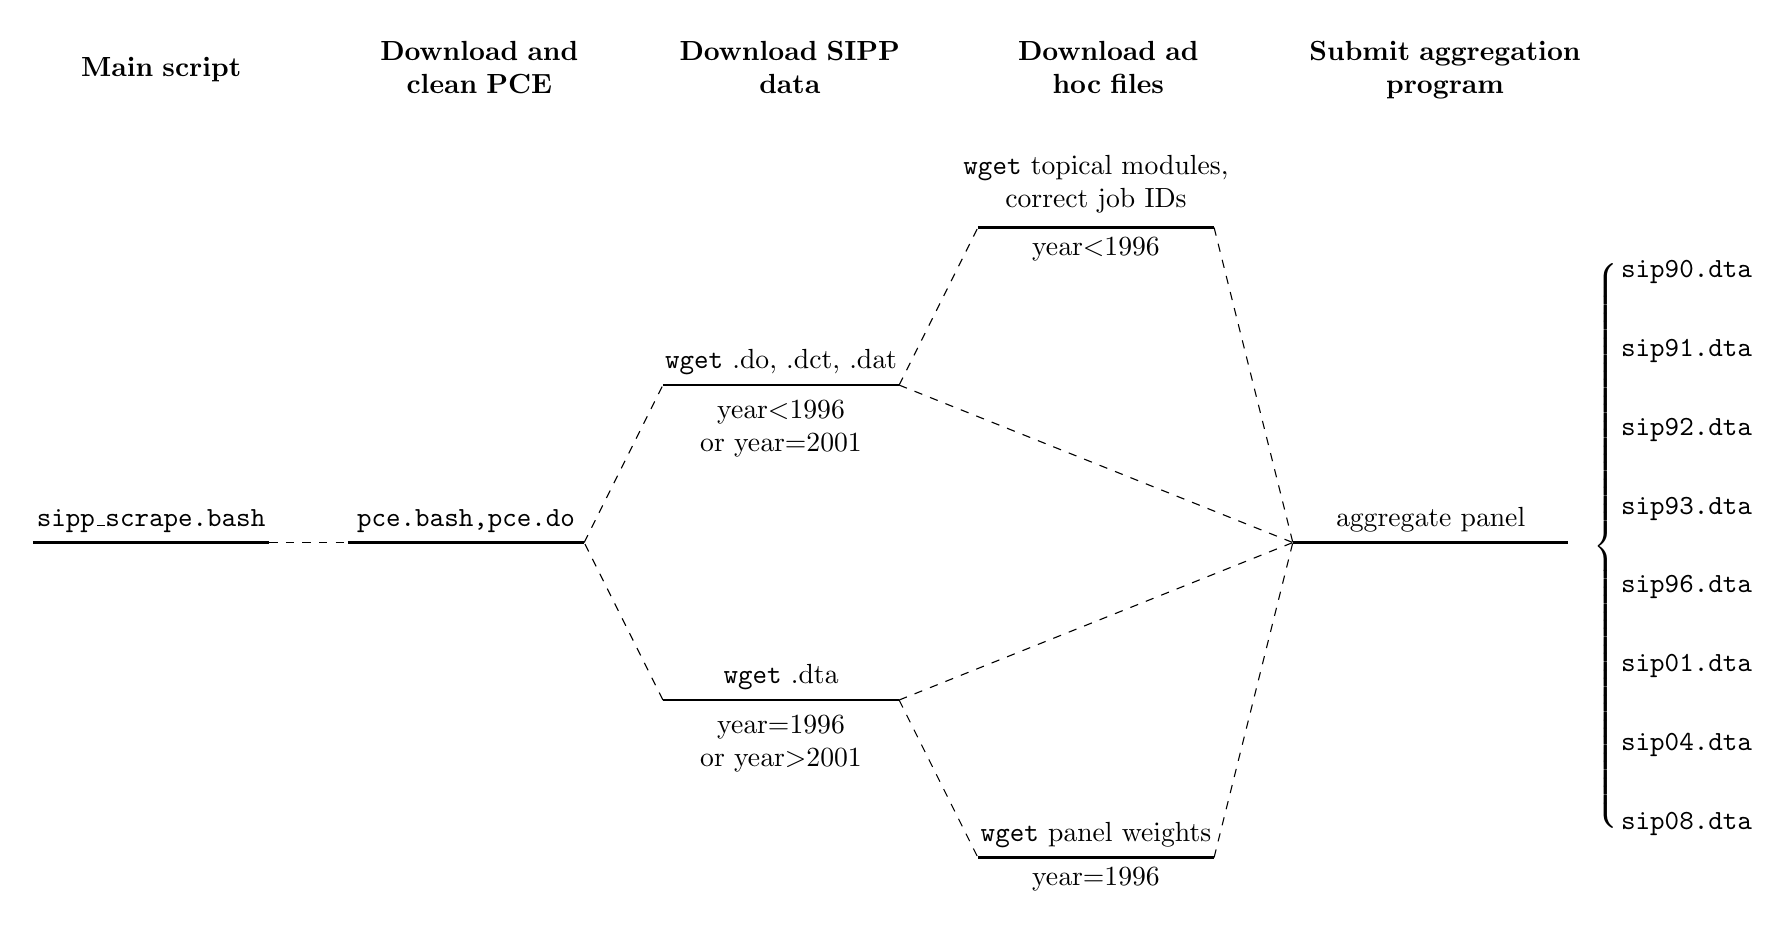
\begin{tikzpicture}
   % Draw all levels
  \draw[level] (0,0) -- node[above] {\tt sipp\_scrape.bash} (3,0);
  \draw[connect] (3,0) -- (4,0);
  \draw[level] (4,0) -- node[above] {\tt pce.bash,\\ pce.do} (7,0);
  \draw[connect] (7,0) -- (8,2) (8,-2) -- (7,0) ;
  \draw[level] (8,2) -- node[above] {{\tt wget} .do, .dct, .dat} node[below] {\begin{tabular}{c} year$<$1996 \\ or year=2001 \end{tabular}} (11,2) ;
  \draw[level] (8,-2) -- node[above] {{\tt wget} .dta} node[below] {\begin{tabular}{c} year=1996 \\ or year$>$2001 \end{tabular}} (11,-2) ;
  \draw[level] (12,4) -- node[above] {\begin{tabular}{c} {\tt wget} topical modules, \\ correct job IDs \end{tabular}} node[below] {year$<$1996 } (15,4) ;
  \draw[level] (12,-4) -- node[above] {{\tt wget} panel weights} node[below] {year=1996 } (15,-4) ;
  \draw[connect] (11,2) -- (12,4);
  \draw[connect] (11,-2) -- (12,-4);
  \draw[level] (16,0) -- node[above] {aggregate panel}  (19.5,0) ;
  \draw[level] (20,0) -- node[below] {\smash{$\left\{\rule{0pt}{105pt}\right.$}}  (20,0) ;
  \draw[connect] (15,4) -- (16,0);
  \draw[connect] (15,-4) -- (16,0);
  \draw[connect] (11,2) -- (16,0);  
  \draw[connect] (11,-2) -- (16,0);
  \draw[level] (21,0) -- node[above, yshift=1ex] {\tt sip93.dta}  (21,0) ;
  \draw[level] (21,1) -- node[above, yshift=1ex] {\tt sip92.dta}  (21,1) ;
  \draw[level] (21,2) -- node[above, yshift=1ex] {\tt sip91.dta}  (21,2) ;
  \draw[level] (21,-1) -- node[above, yshift=1ex] {\tt sip96.dta}  (21,-1) ;
  \draw[level] (21,-2) -- node[above, yshift=1ex] {\tt sip01.dta}  (21,-2) ;
  \draw[level] (21,-3) -- node[above, yshift=1ex] {\tt sip04.dta}  (21,-3) ;
  \draw[level] (21,-4) -- node[above, yshift=1ex] {\tt sip08.dta}  (21,-4) ;
  \draw[level] (21,3) -- node[above, yshift=1ex] {\tt sip90.dta}  (21,3) ;
  % Draw labels
  \node[label] at (1.9,6)  {\bf \begin{tabular}{c}Main script \end{tabular}};
  \node[label] at (5.7,6)  {\bf\begin{tabular}{c} Download and \\ clean PCE \end{tabular}};
  \node[label] at (9.5,6)  {\bf\begin{tabular}{c} Download SIPP \\ data \end{tabular}};
  \node[label] at (13.8,6)  {\bf\begin{tabular}{c} Download ad \\ hoc files \end{tabular}};
  \node[label] at (17.5,6)  {\bf\begin{tabular}{c} Submit aggregation \\ program \end{tabular}};
\end{tikzpicture}
\end{landscape}

\newpage
\newgeometry{left=1in, right=1in, bottom=1.5in, top=1.5in}
\section{Instructions for Running Bash Script}\label{sec:instructions}
In general, the only thing that changes across operating systems is the way 
\subsection{Linux}
	\begin{itemize}
	\item Make sure {\tt wget} is installed
	\item {\tt os} should be set to ``{\tt linux}'' in the user options section
	\item Populate other user options according to user-specific details
	\end{itemize}
\subsection{Mac}
	\begin{itemize}
	\item {\tt os} should be set to ``{\tt mac}'' in the user options section
	\item Make sure you can submit .do files in batch mode. Open Terminal and type ``{\tt bash}", ``{\tt echo \$PATH}"
	\item If you don't see ``{\tt /Applications/Stata/Stata\{MP/SE\}.app/Contents/MacOS/.}'' then type\\ ``{\tt export 			PATH=\$\{PATH\}:/Applications/Stata/Stata\{MP/SE\}.app/Contents/MacOS/.}'' (be sure to replace the MP/SE with whatever Stata package you're running)
	\item You should now be able to run Stata in batch mode if by calling {\tt stata -b do} (so populate the {\tt stata} parameter with that)
	\item Populate other user options according to user-specific details
	\end{itemize}
\subsection{Windows}
	\begin{itemize}
	\item {\tt os} should be set to ``{\tt windows}'' in the user options section
	\item Make sure {\tt wget} is installed and specify the {\tt stata} parameter correctly (see below)
	\item Calling Stata from batch mode can be done by specifying where the Stata executable file resides on your machine. For example: \\
	{\tt ``C:{\textbackslash}Program Files (x86){\textbackslash}Stata13{\textbackslash}StataSE-64'' -e do test.do}\\
	would work. The ``{\tt -e}'' option here forces Stata to run in the background and print everything to a ``{\tt test.log}'' file.
	\item Populate other user options according to user-specific details
	\end{itemize}


\end{document}